% Possible values for aspect ratio are: 169, 1610, 149, 54, 43 and 32.
\documentclass[aspectratio=1610]{beamer}
\usetheme{cern}

% Change bullet points
\usepackage{enumitem}
\setbeamertemplate{itemize items}[square]
\setitemize{label=\raisebox{0.3ex}{\usebeamerfont*{itemize item}
\usebeamercolor[fg]{itemize item}
\usebeamertemplate{itemize item}}}
%\setlist[itemize]{leftmargin=*, itemsep=0pt, parsep=2pt, labelsep*=2em, labelindent=0em, before=\vspace{-\dimexpr\baselineskip +2.6\partopsep}}

% CERN blue is Pantone 286 = RGB 56 97 170, defined as cern@blue below
\definecolor{cern@ltblue}{rgb}{0.415686,0.611765,0.964706} % RGB 106 156 246
\definecolor{cern@blue}  {rgb}{0.219608,0.380392,0.666667} % RGB  56  97 170
\definecolor{cern@dkblue}{rgb}{0.082353,0.184314,0.364706} % RGB  21  47  93

% Complimentary colours
\definecolor{cern@ltcomp}{rgb}{0.666667,0.525490,0.219608} % RGB 170 134  56
\definecolor{cern@dkcomp}{rgb}{0.364706,0.266667,0.047059} % RGB  93  68  12

%\setbeamercolor{title}               {bg=cern@blue,fg=white}
%\setbeamercolor{frametitle}          {bg=cern@blue,fg=white}
%\setbeamercolor{section in head/foot}{bg=cern@ltblue,fg=white}
\setbeamercolor{itemize item}         {fg=cern@dkcomp}
\setbeamerfont{itemize item}          {size=\large}



%%
%% Get packages that we need
%%

% Adjust page margins on-the-fly
\usepackage{changepage}

% Change fonts to Avenir
% Note: need to compile with xelatex to use this package
\usepackage{fontspec}
\setsansfont{AvenirLTStd-Book}

\usepackage[showboxes,overlay,absolute]{textpos}
\usepackage[overlay,absolute]{textpos}
\setlength{\TPHorizModule}{.01\paperwidth} % Horizontal units are percent of paper width
\setlength{\TPVertModule}{.01\paperwidth}  % Make vertical units equal to horizontal units
\textblockorigin{.5\paperwidth}{4.25ex}

% Headings within slides
\usepackage{xcolor}
\usepackage{tabularx}



%%
%% Title page
%%

\author{\Large Dr. Michael Davis for the CTA Team}
\title[Migrating to CTA]{Migrating from CASTOR\\
to the new\\
CERN Tape Archive (CTA)\\}
\date{17 February 2020}

\begin{document}

\frame{\titlepage}

\begin{frame}{Presenting the CERN Tape Archive (CTA)}
   \centering
   \includegraphics<1>[width=0.75\textwidth]{../../Logo/Logo_CERN_Tape_Archive}
   \includegraphics<2>[width=\textwidth]{../../Logo/Logo_EOS+CTA}
   \includegraphics<3>[width=\textwidth]{images/Love_EOS+CTA}
   \vspace{1cm}
   \only<2>{\LARGE\centering CTA is the tape back-end to EOS}
   \only<3>{\LARGE\centering FTS+EOS+CTA = {\color{red}$\heartsuit$}}
\end{frame}

\begin{frame}{EOS+CTA in Production by End 1Q 2020}
   \centering
   
\includegraphics[width=\textwidth]{images/CASTOR_EOS+CTA_Logo}
\end{frame}

\begin{frame}{\only<1>{CASTOR \color{cern@ltblue}vs. EOS+CTA}\only<2>{{\color{cern@ltblue}CASTOR vs.} EOS+CTA}}
   \centering
   \vspace{1ex}
   \includegraphics<1>[width=0.75\textwidth]{images/CASTOR_Arch}
   \includegraphics<2>[width=0.75\textwidth]{images/CTA_Arch}
\end{frame}

\begin{frame}{EOS+CTA : Who Does What?}{}
   \renewcommand{\arraystretch}{1.1}
   \begin{tabularx}{\textwidth}{>{\raggedright}X>{\raggedright\arraybackslash}c}
        \multicolumn{1}{c}{\fontspec{Humanst521 BT}\color{cern@blue}Function}
      & \multicolumn{1}{c}{\fontspec{Humanst521 BT}\color{cern@blue}Provided by}\\[0.5ex]
      \hline
      File Metadata Operations & EOS\\
      Namespace & EOS\\
      Disk Buffer for Staging & EOS\\
      \hline
      Tape File Metadata Ops & CTA\\
      % CTA does not know the filename of a file. If you give it a fileid, it can tell you its size
      % and checksum, how many copies there are and which tapes the copies are stored on.
      Archive/Recall Requests & CTA\\
      Tape File Catalogue & CTA\\
      Tape Operations (libraries, drives, cassettes) & CTA\\
   \end{tabularx}
% Main difference with CASTOR: EOSCTA is a pure tape system.
\end{frame}

\begin{frame}{EOS+CTA : ``Best of Both Worlds''}
   \begin{itemize}
       \item EOS provides the interface, file operations and namespace
       \item CTA provides highly performant tape operations\\
          based on CASTOR Tape Server\\[2ex]
   \end{itemize}
   {\LARGE\color{cern@blue}CTA Design Principles}
   \begin{itemize}
      \item Simplicity
      \item Scalabilty
      \item Performance
   \end{itemize}
\end{frame}

\begin{frame}{EOS+CTA Performance Enhancements}{}
% to manage how and when tapes will be mounted, to optimise the use of the tape infrastructure.

% mention in the beginning for the audience why castor -> CTA, saying how good was castor, how well it worked,
% but mention that it was stretching itself to the limits, we have now almost an order of magnitude of GB/s
% to/from tape to handle, we had "problems" with the fragmentation of stager etc,
   {\color{cern@blue}Reduced latency compared to CASTOR}
\begin{itemize}
   \item Advanced queue manager\\
   \item Just-in-time scheduling\\[2ex]
\end{itemize}
   {\color{cern@blue}New features in the pipeline}
\begin{itemize}
   \item Preemptive scheduling
   \item Recommended Access Order (RAO) for LTO media
   \item Colocation hints
\end{itemize}
\end{frame}

\begin{frame}{Data Management Stack}
\begin{columns}
	\begin{column}{0.4\textwidth}
		\begin{center}
         \includegraphics[width=\textwidth]{images/CTA_Deployment}
		\end{center}
	\end{column}
	\begin{column}{0.55\textwidth}
      {\color{cern@blue}``Big EOS''}
      {\small
\begin{itemize}
        \item Tens of PB of storage for reconstruction, analysis and staging to Tier--1s
        \item Accounted as part of the pledge
\end{itemize}
      }
      {\color{cern@blue}``Little EOS''}
      {\small
		\begin{itemize}
        \item Small buffer for copying files to/from tape
        \item Not part of the pledge; not available for physics jobs
        \item Files are deleted as soon as they are safely archived on tape or
           copied to ``Big EOS''
        \item SSDs: reduce contention and give the best price/performance ratio
		\end{itemize}
      }
	\end{column}
\end{columns}
\end{frame}

\begin{frame}{Max. throughput, minimum contention}
  \centering
  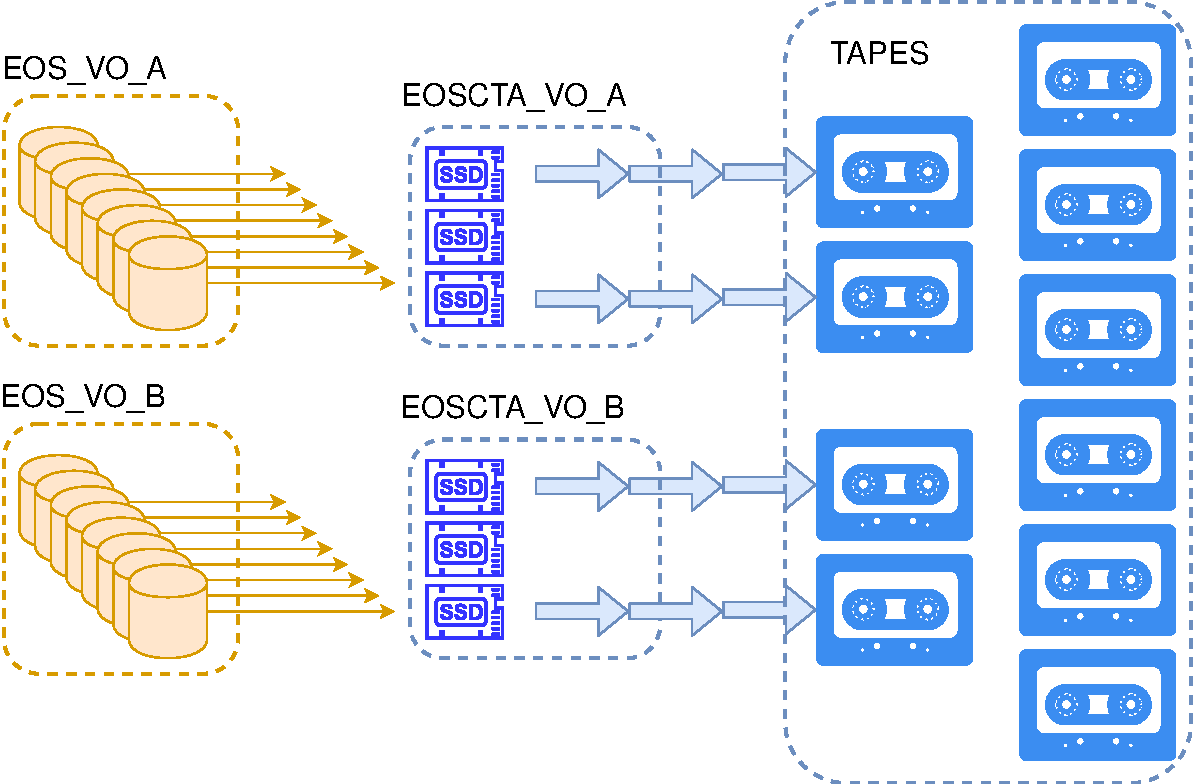
\includegraphics[width=0.7\textwidth]{images/upload_e764d94a4ee3ac79c328ea0d21a6a128.pdf}
\end{frame}

\begin{frame}{EOS+CTA Production Status : Hardware}
   {\LARGE\color{cern@blue}Hardware is Installed and Ready}
   \begin{itemize}
      \item 6$\times$ 100 Gb/s network links
      \item 32$\times$ hyper-converged servers
      \begin{itemize}
         \item 16$\times$ 2 TB SSD
         \item 25 Gb/s Ethernet
      \end{itemize}
      \item 29$\times$ Tape Drives
   \end{itemize}
% 24x 2.5" hot-swappable SSD slots
% 2x Intel Xeon Scalable 5218 processors
% 192GB of DDR4 ECC Reg memory running at 2667 MHz (M393A2K43BB1-CTD)
% 1x 512GB Samsung 970 EVO Plus NVMe SSD for OS (MZ-V7P512BW)
% 16x 1.92TB Intel S4510 SSD (SSDSC2KB019T801) running firmware >= XCV10110
% 2x 25Gbit/s Ethernet ports and 1x dedicated management port
\end{frame}

\begin{frame}{EOS+CTA Production Status : Software}
   \begin{itemize}
      \item CTA version 1.1 deployed
      \item Archival/retrieval workflows integrated with ATLAS\\
         (FTS and Rucio)
      \item Integration with ATLAS SFO has started
   \end{itemize}
\end{frame}

\begin{frame}{EOS+CTA Status : Commissioning}{}
% On Tue 21st Atlas started a major reprocessing campaign, scheduled to recall 4PB of data from a
% production instance of CTA. The service has performed well so far, reaching sustained throughput of
% 5GB/s, limited in this case by the network interfaces of the CTA nodes. More nodes will be added in
% order to demonstrate the horizontal scaling of the service.
   \centering
   \vspace{1ex}
   {\LARGE\color{cern@blue}ATLAS Reprocessing Campaign :\\
   1 PB recalled @ 4 GB/s}

\begin{adjustwidth}{-1cm}{-1cm}
   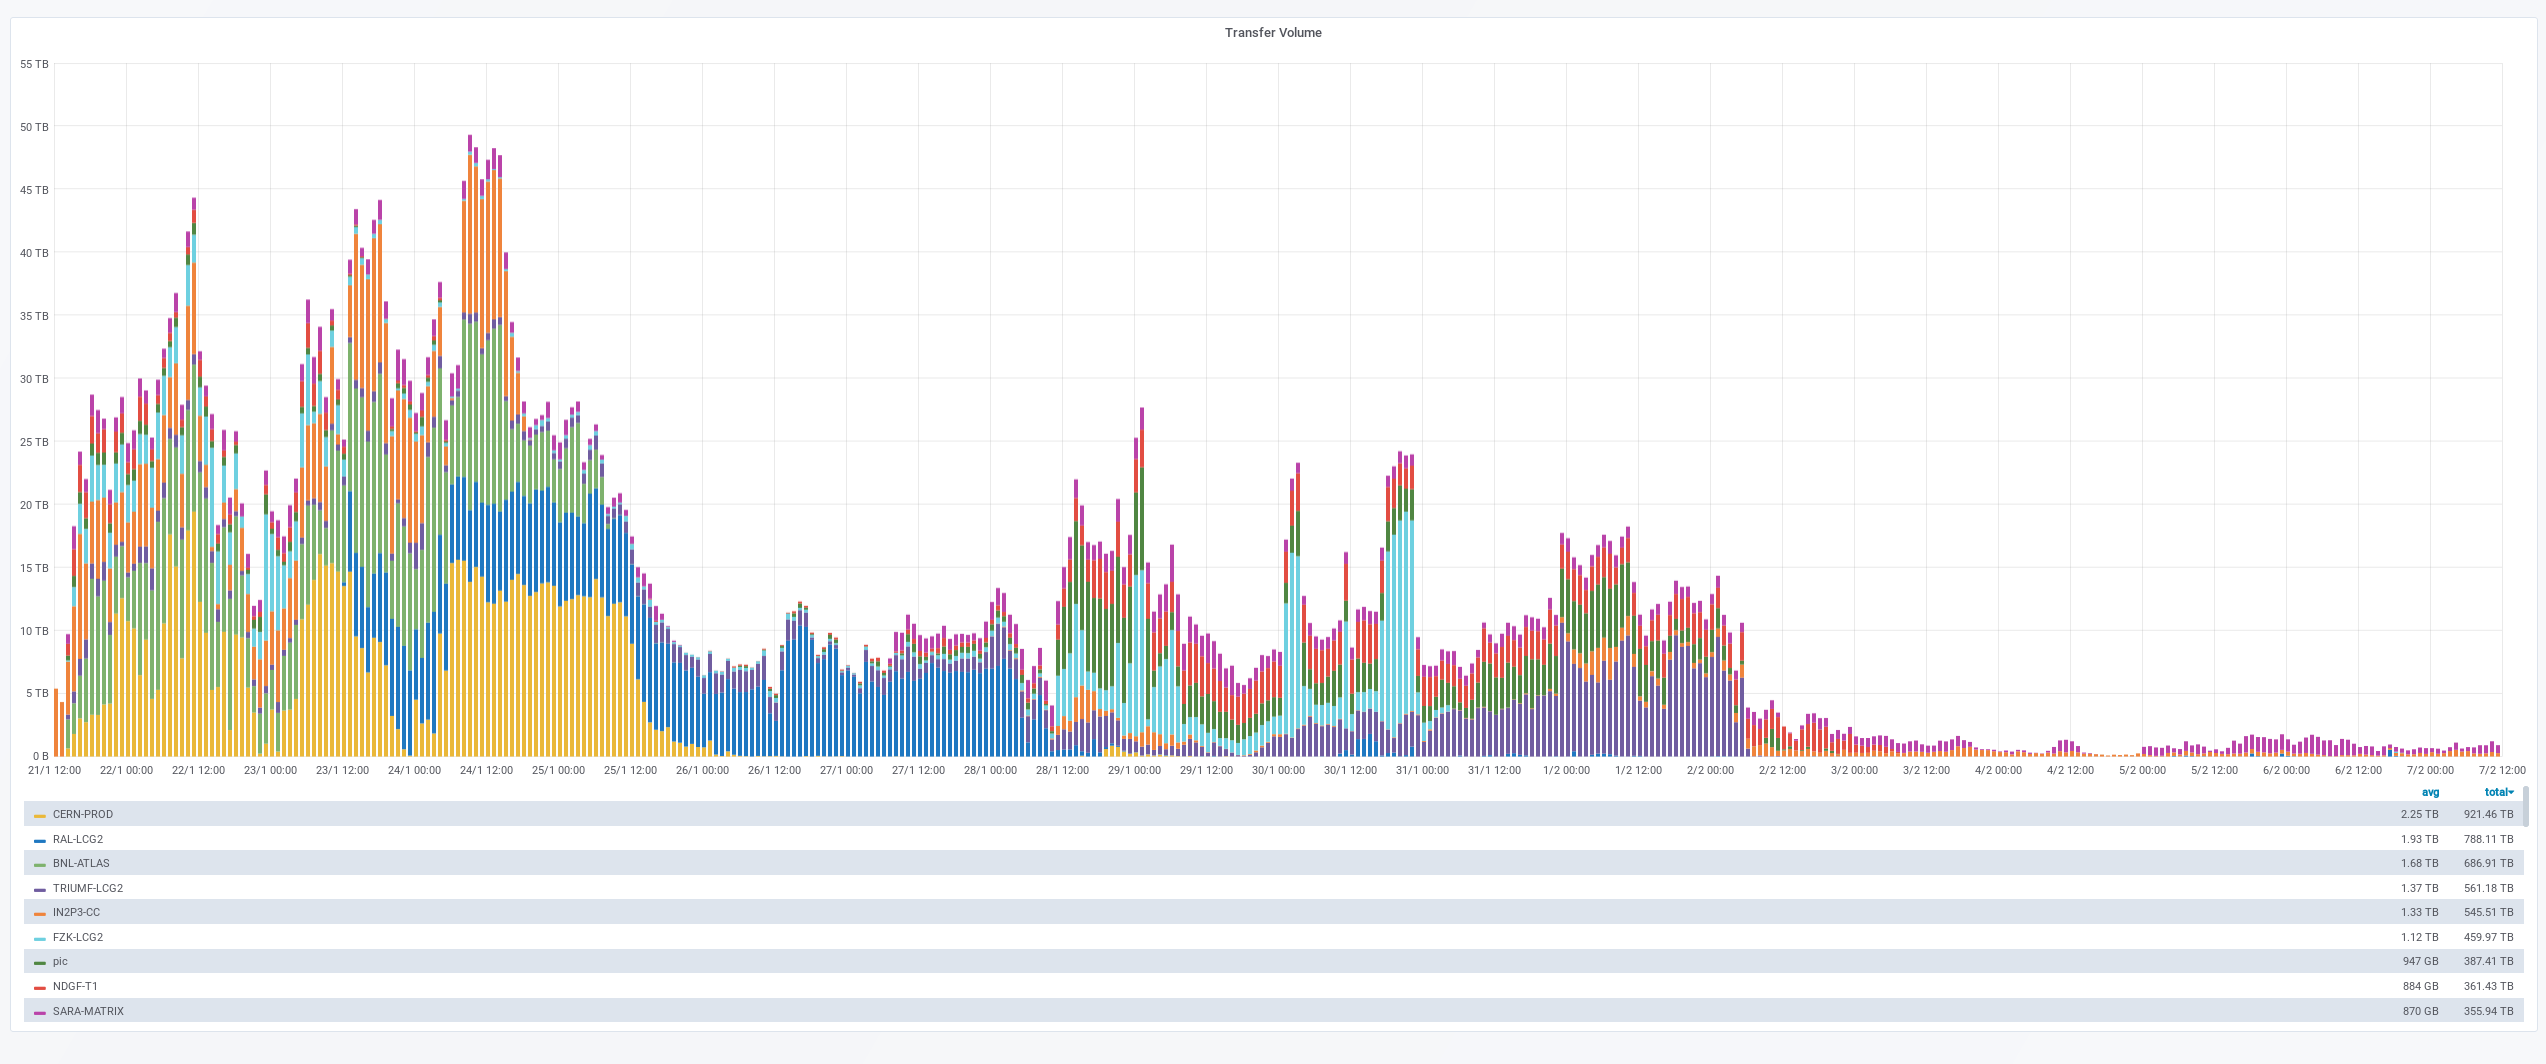
\includegraphics[width=\linewidth]{images/RecallTest}
\end{adjustwidth}
\end{frame}

\begin{frame}{EOS+CTA Status : Commissioning}{}
   \centering
   \vspace{1ex}
   {\LARGE\color{cern@blue}ATLAS Write Stress Test : 0.6 PB at\\
   sustained 5.6 GB/s (17 tape drives in parallel)\\[1ex]}

   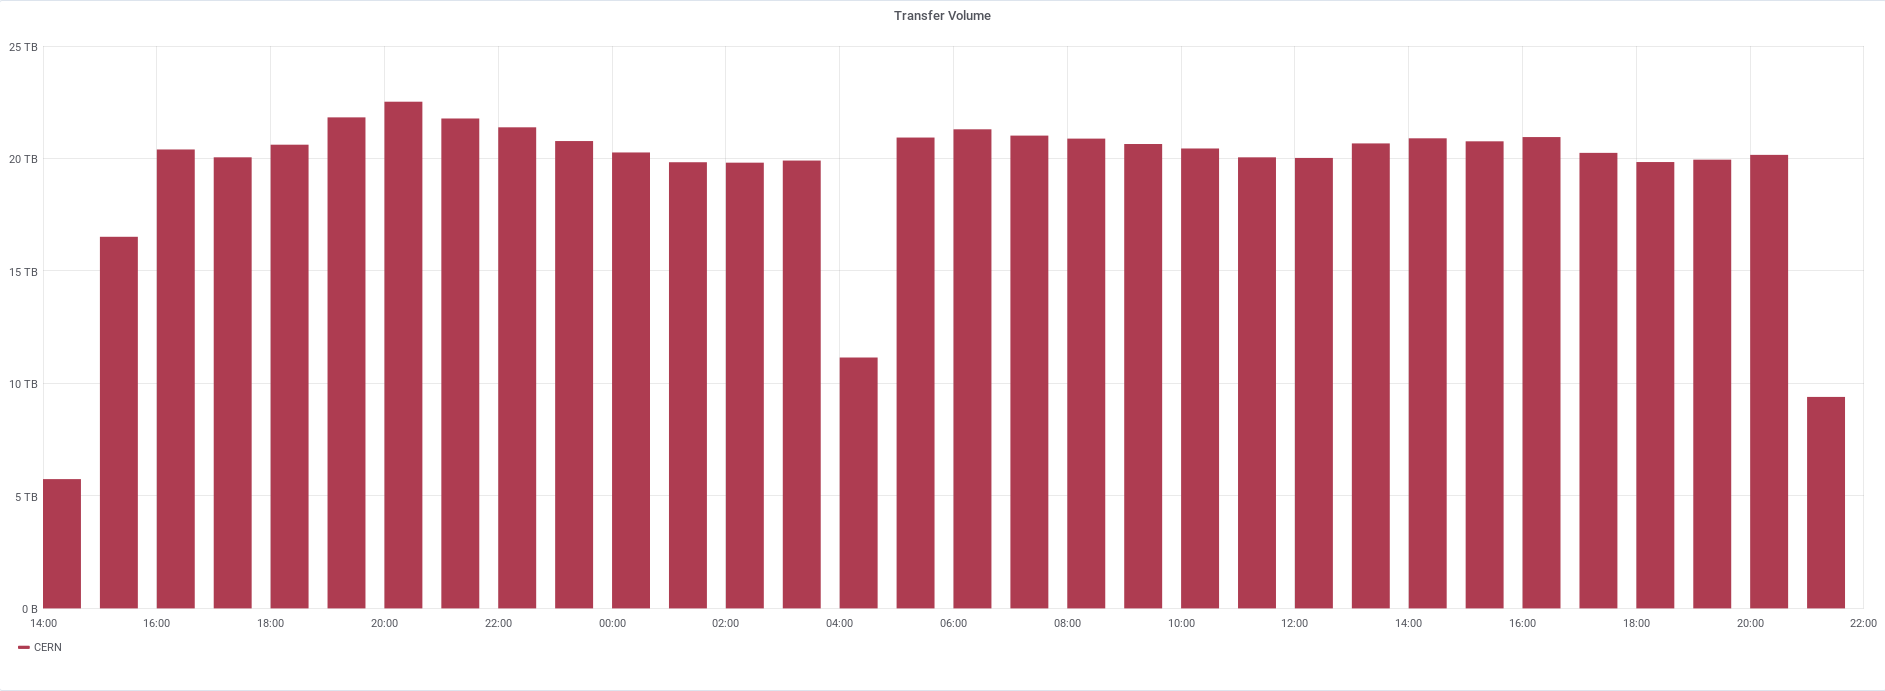
\includegraphics[width=\linewidth]{images/WriteStressTest}
\end{frame}

\begin{frame}{EOS+CTA Status : Commissioning}{}
% I would not stick on dates as written on stones. good to have exact day, but mention "tentative"and possibility of being flexible in case is needed.
   \begin{itemize}
      \item Limiting factor on throughput was hardware and network bandwidth
      \item Software scaled smoothly as more hardware was added
      \item Final ATLAS acceptance tests during March
   \end{itemize}
\end{frame}

\begin{frame}{Migration from CASTOR to CTA}{}
   {\color{cern@blue}Migration is a Metadata-only Operation}
   \begin{itemize}
      \item Tape file format between CASTOR and CTA is identical
      \item No physical rewriting of data
      \item Migration process has been tested many times (including ATLAS recall exercises in 2019 and 2020)\\[1ex]
   \end{itemize}

   {\color{cern@blue}Risk Mitigation}
   \begin{itemize}
      \item Tapes imported from CASTOR are read-only in CTA
      \item To return a tape to CASTOR : disable the tape in the CTA catalogue and re-enable the tape in CASTOR
   \end{itemize}
\end{frame}

\begin{frame}{EOS+CTA Deployment}
   \begin{itemize}
      \item 4 instances for the LHC experiments
      \item 1 instance for PUBLIC
      \begin{itemize}
         \item Active non-LHC experiments :\\
            \textit{AMS, Compass, Dune, NA61, NA62, nTOF, \ldots}
         \item Inactive legacy experiments: \textit{LEP, \ldots}
         \item User files
      \end{itemize}
   \item Tier--1s: \textit{RAL}
   \end{itemize}
\end{frame}

\begin{frame}{ATLAS Migration (1Q 2020)}
\begin{columns}
	\begin{column}{0.4\textwidth}
		\begin{center}
         \includegraphics[width=\textwidth]{images/CTA_Deployment_Atlas}
		\end{center}
	\end{column}
	\begin{column}{0.55\textwidth}
   \begin{itemize}
      \item Rucio + FTS + EOS + CTA
      \item Subject to satisfactory test results, EOSCTAATLAS will go into production end of March 2020
      \item CASTOR ATLAS will be disabled after the migration
   \end{itemize}
	\end{column}
\end{columns}
\end{frame}

\begin{frame}{ALICE Migration (2Q 2020)}
\begin{columns}
	\begin{column}{0.4\textwidth}
		\begin{center}
		  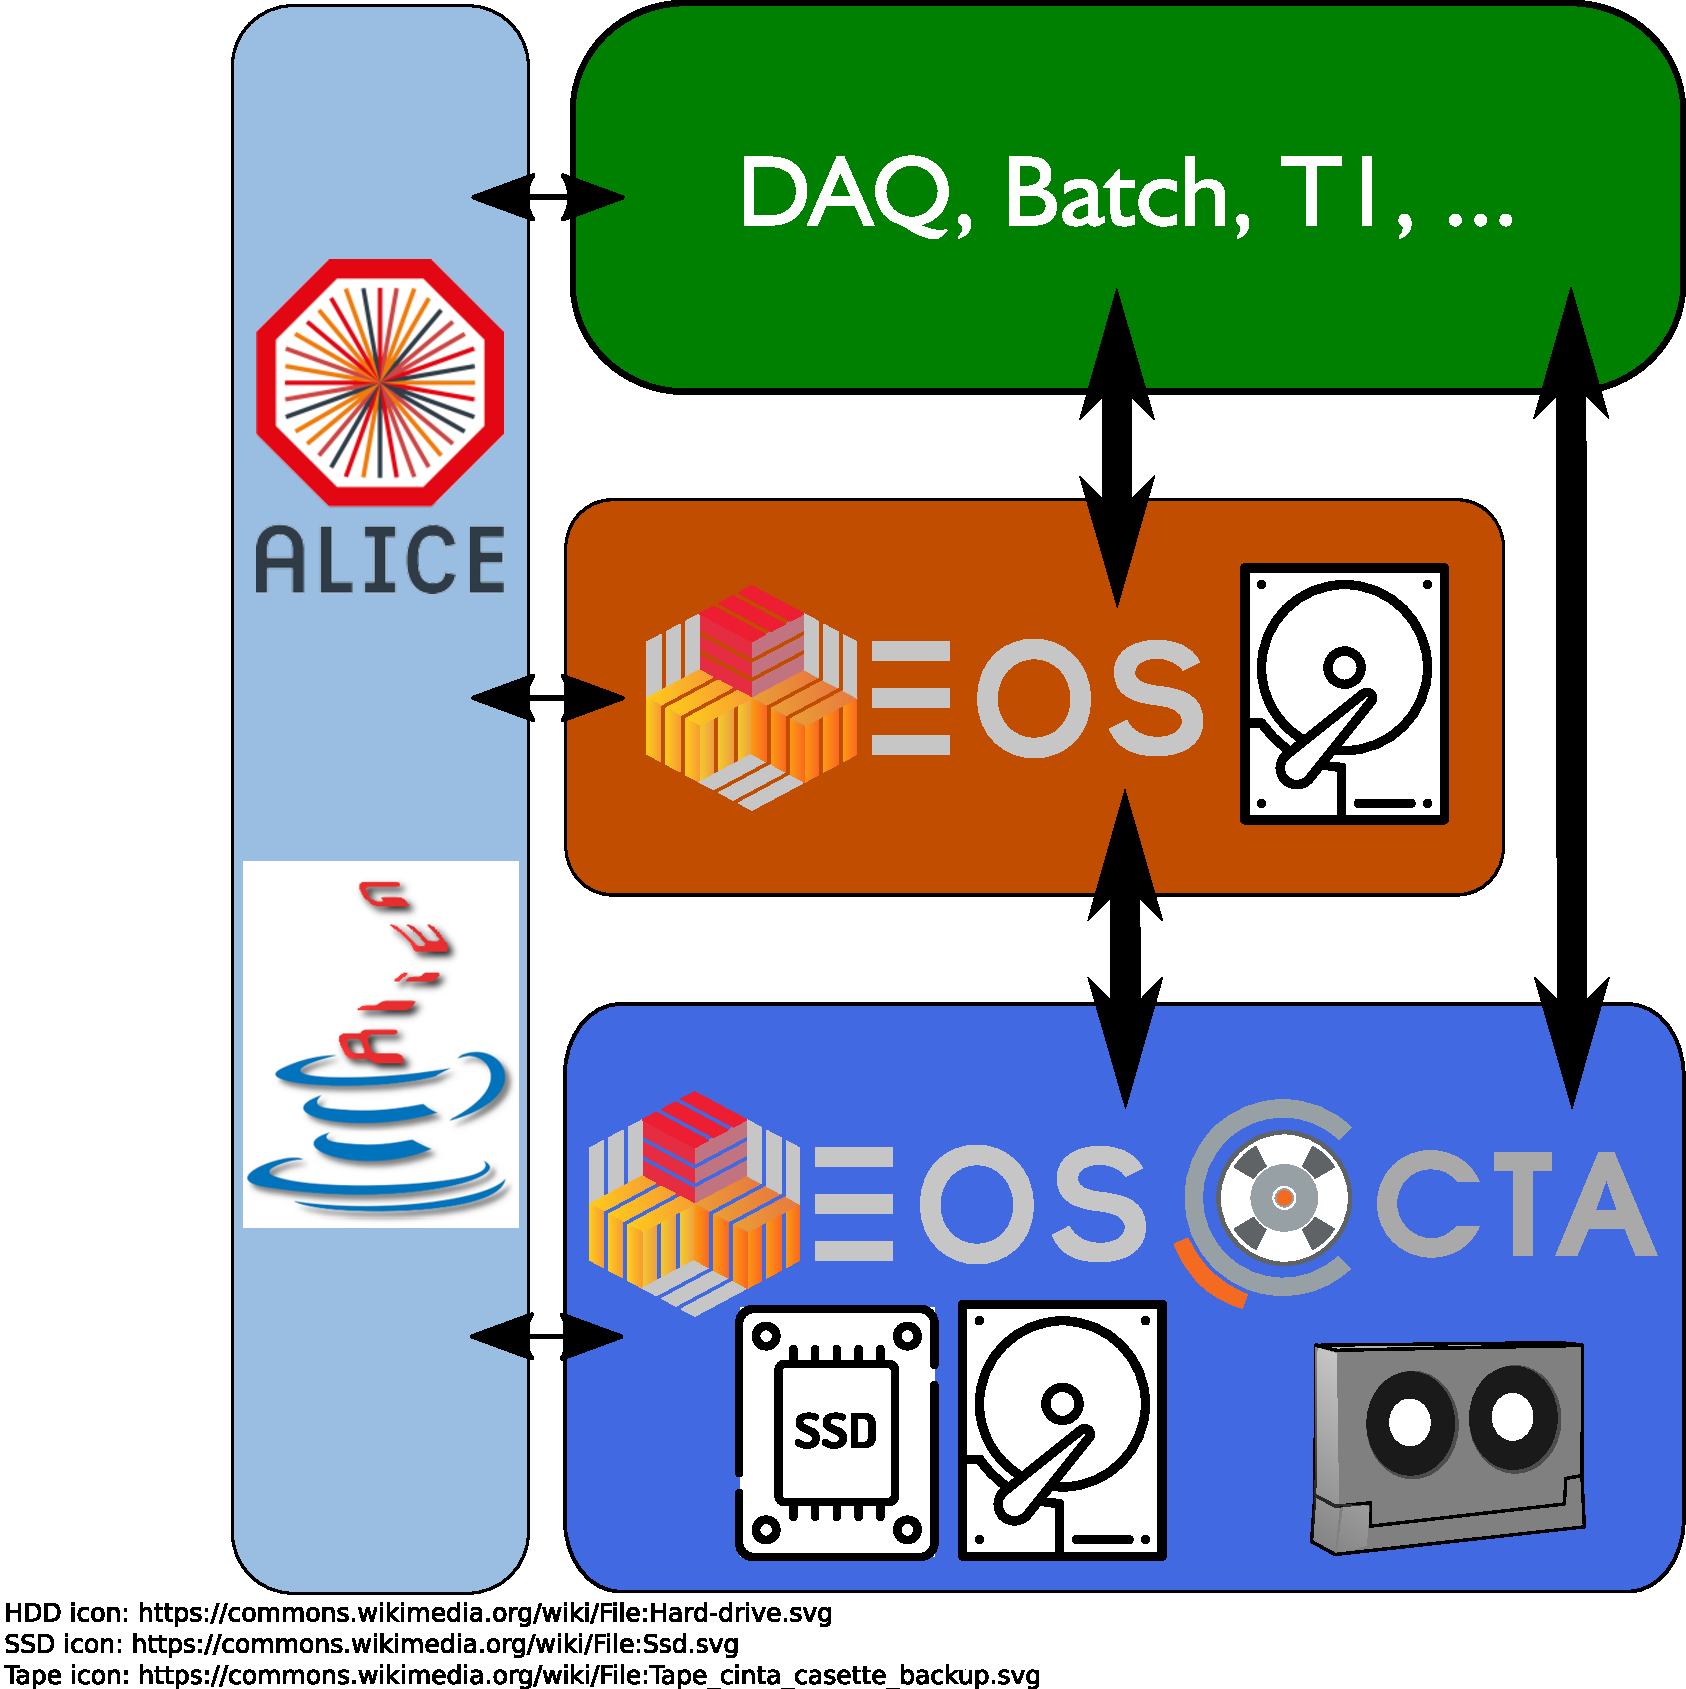
\includegraphics[width=\textwidth]{images/CTA_Deployment_ALICE.pdf}
		\end{center}
	\end{column}
	\begin{column}{0.55\textwidth}
      Schedule to be agreed with ALICE\\[1ex]
		\begin{itemize}
         \item JAlien + EOS + CTA
         \item Dual Space buffer
		\begin{itemize}
		  \item SSD buffer for data taking
		  \item $\approx$5 PB HDD cache for retrieves, with garbage collection
		\end{itemize}
		  \item Requirement for occasional T1 access to EOSCTA
		\end{itemize}
	\end{column}
\end{columns}
\end{frame}

\begin{frame}{CMS Migration (2H 2020)}
\begin{columns}
	\begin{column}{0.4\textwidth}
		\begin{center}
		  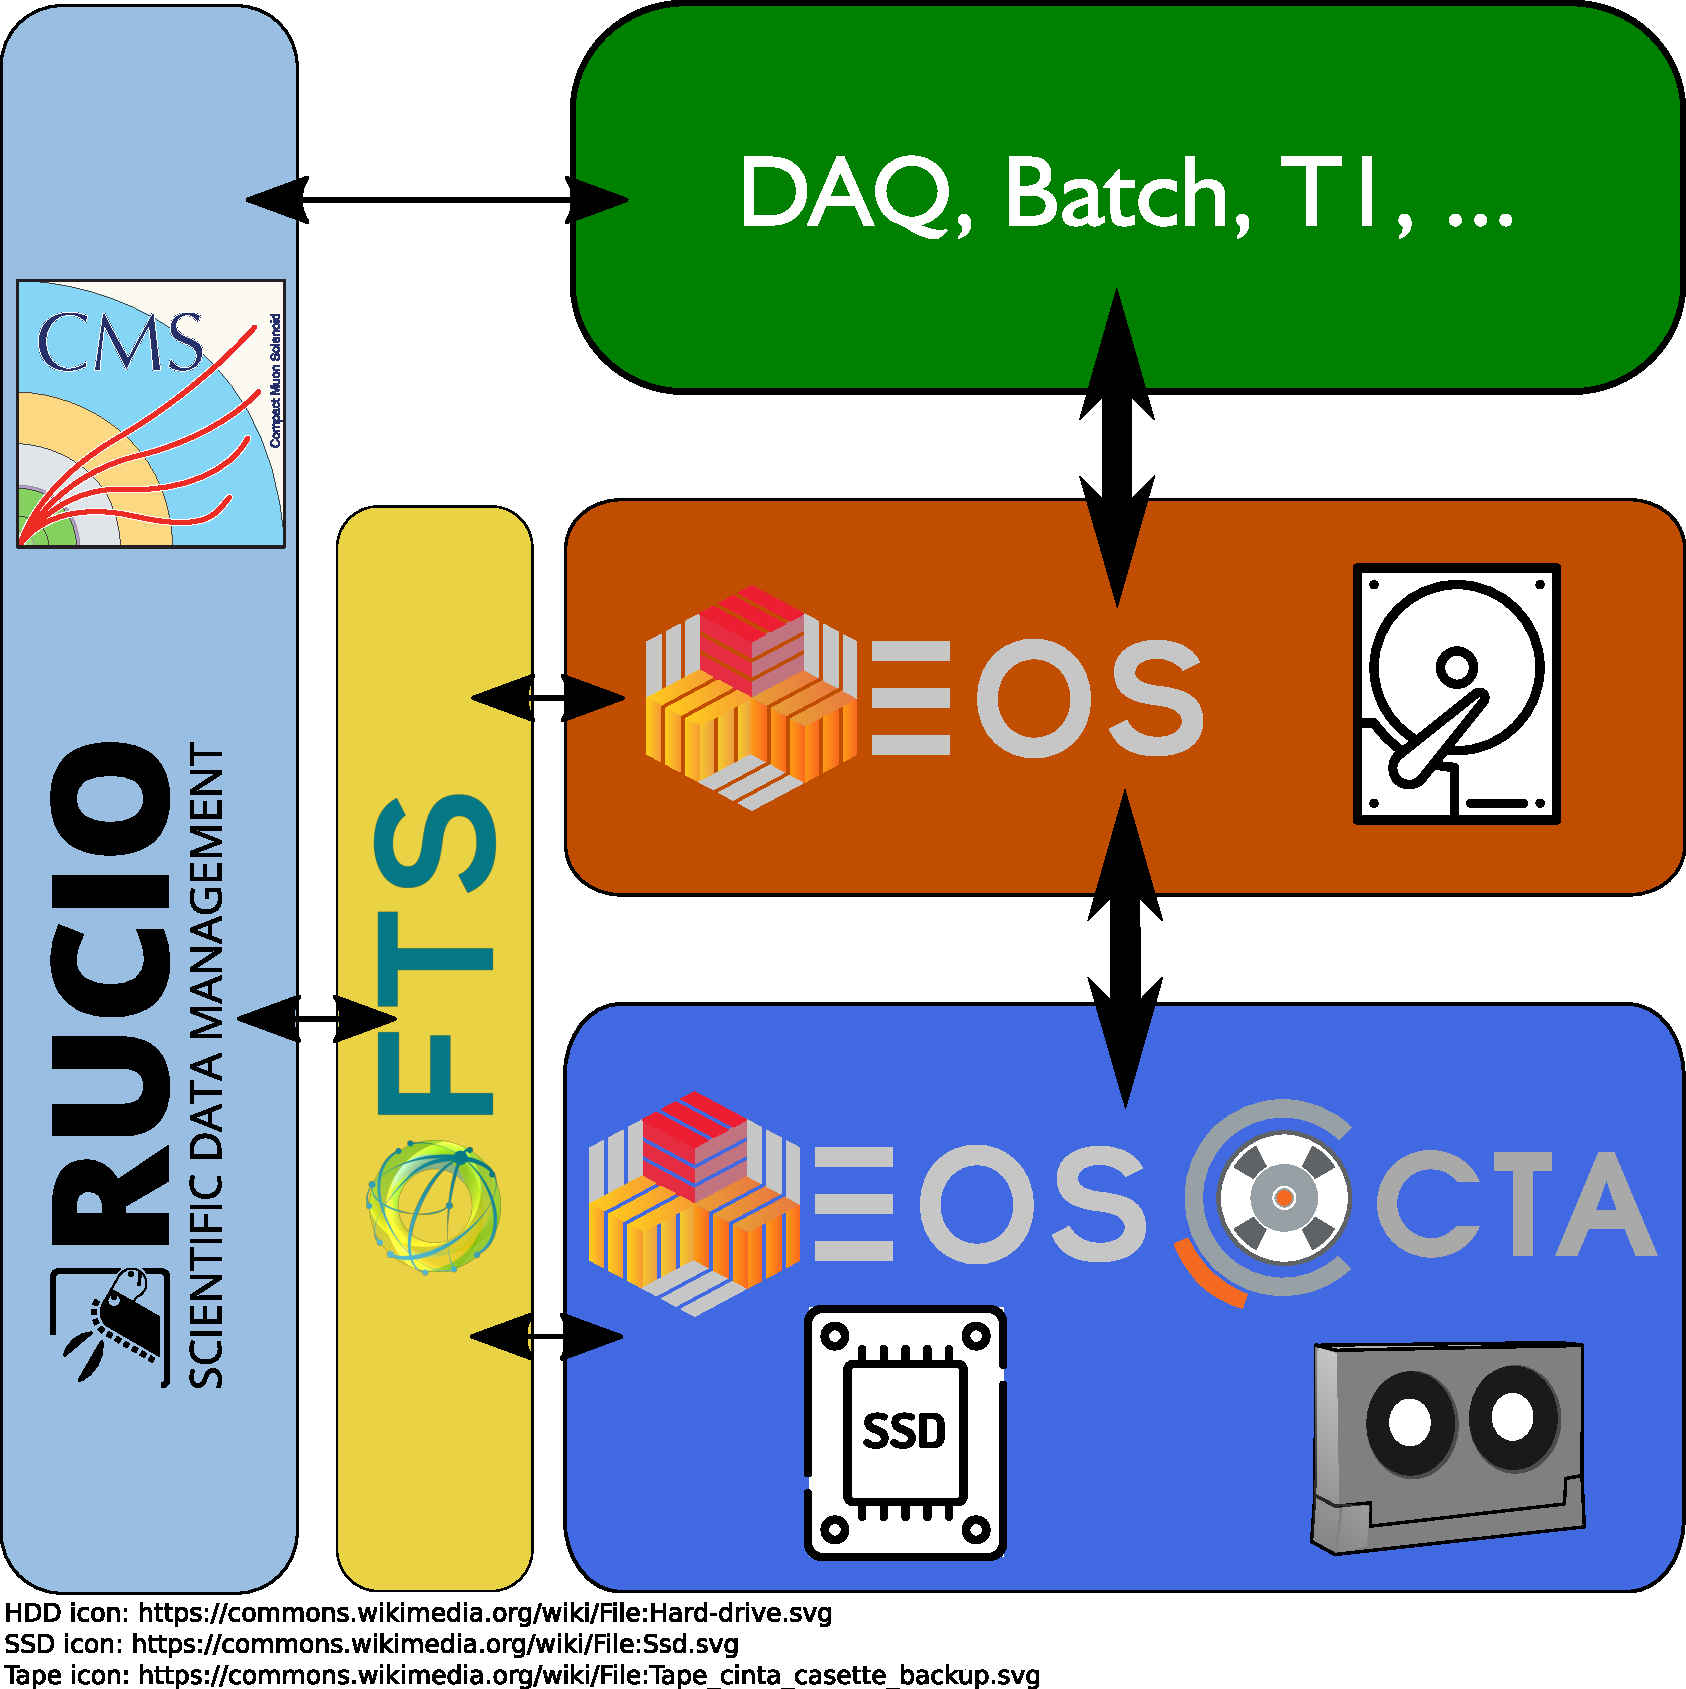
\includegraphics[width=\textwidth]{images/CTA_Deployment_CMS.pdf}
		\end{center}
	\end{column}
	\begin{column}{0.55\textwidth}
		\begin{itemize}
		  \item Similar setup to ATLAS : Rucio + FTS + EOS + CTA
        \item Schedule driven by CMS adoption of Rucio
		\end{itemize}
	\end{column}
\end{columns}
\end{frame}

\begin{frame}{LHCb Migration (2H 2020)}
\begin{columns}
	\begin{column}{0.4\textwidth}
		\begin{center}
		  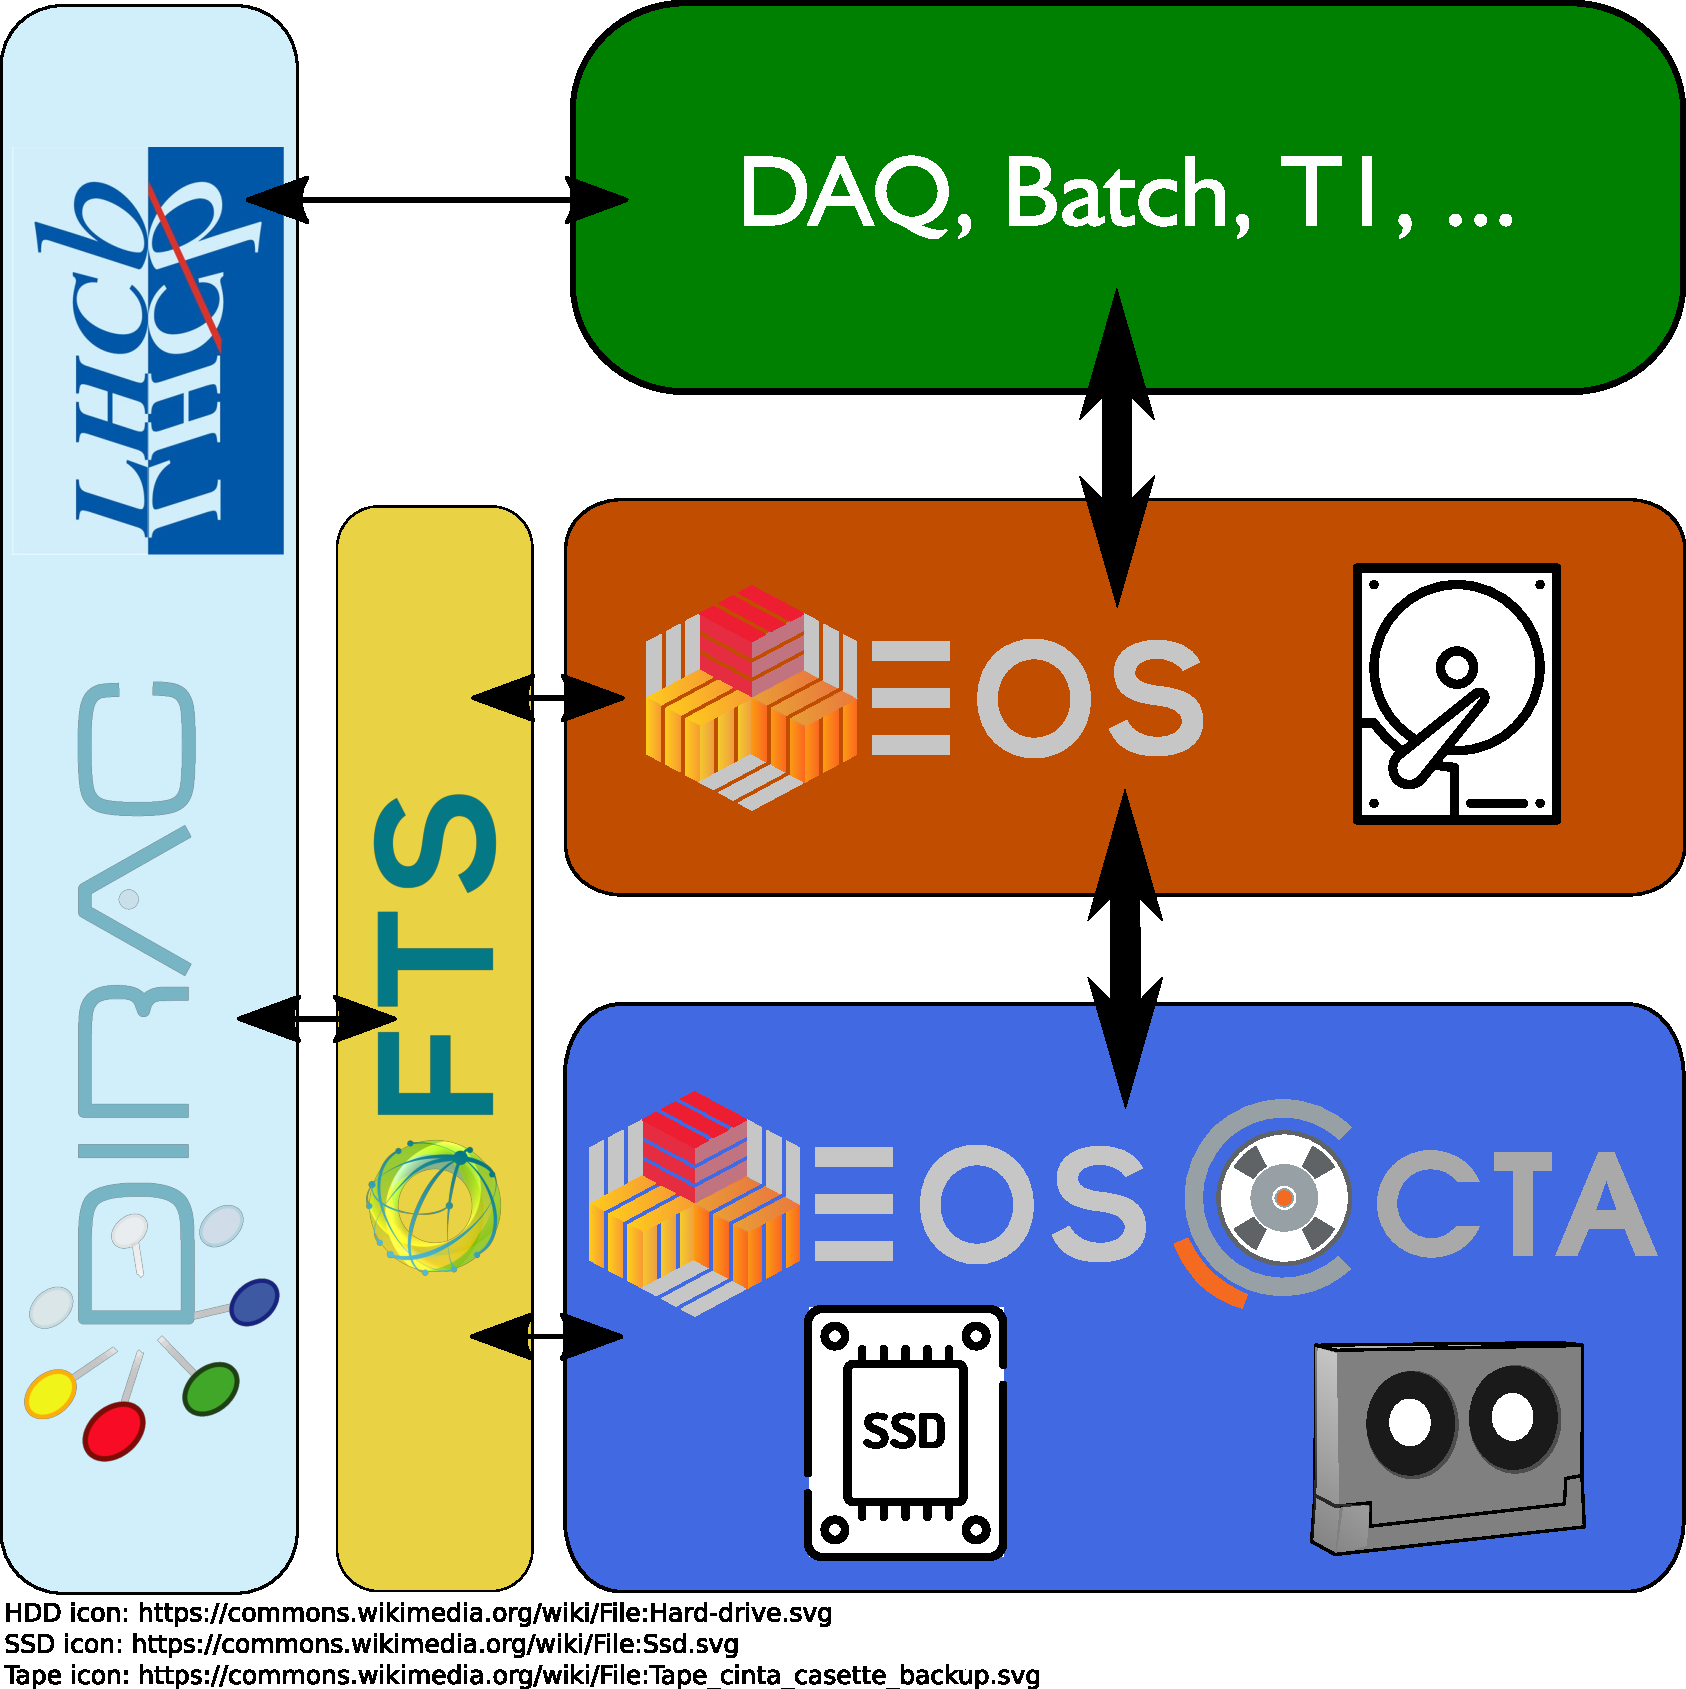
\includegraphics[width=\textwidth]{images/CTA_Deployment_LHCb.pdf}
		\end{center}
	\end{column}
	\begin{column}{0.55\textwidth}
		\begin{itemize}
		  \item Similar setup to ATLAS and CMS : Dirac + FTS + EOS + CTA
		  \item Requirement for occasional export from EOSCTA to T1
        \item Schedule driven by T1s supporting XRootD 3rd Party Copy with delegation
		\end{itemize}
	\end{column}
\end{columns}
\end{frame}

\begin{frame}{Non-LHC Experiments}
\begin{columns}
	\begin{column}{0.4\textwidth}
		\begin{center}
		  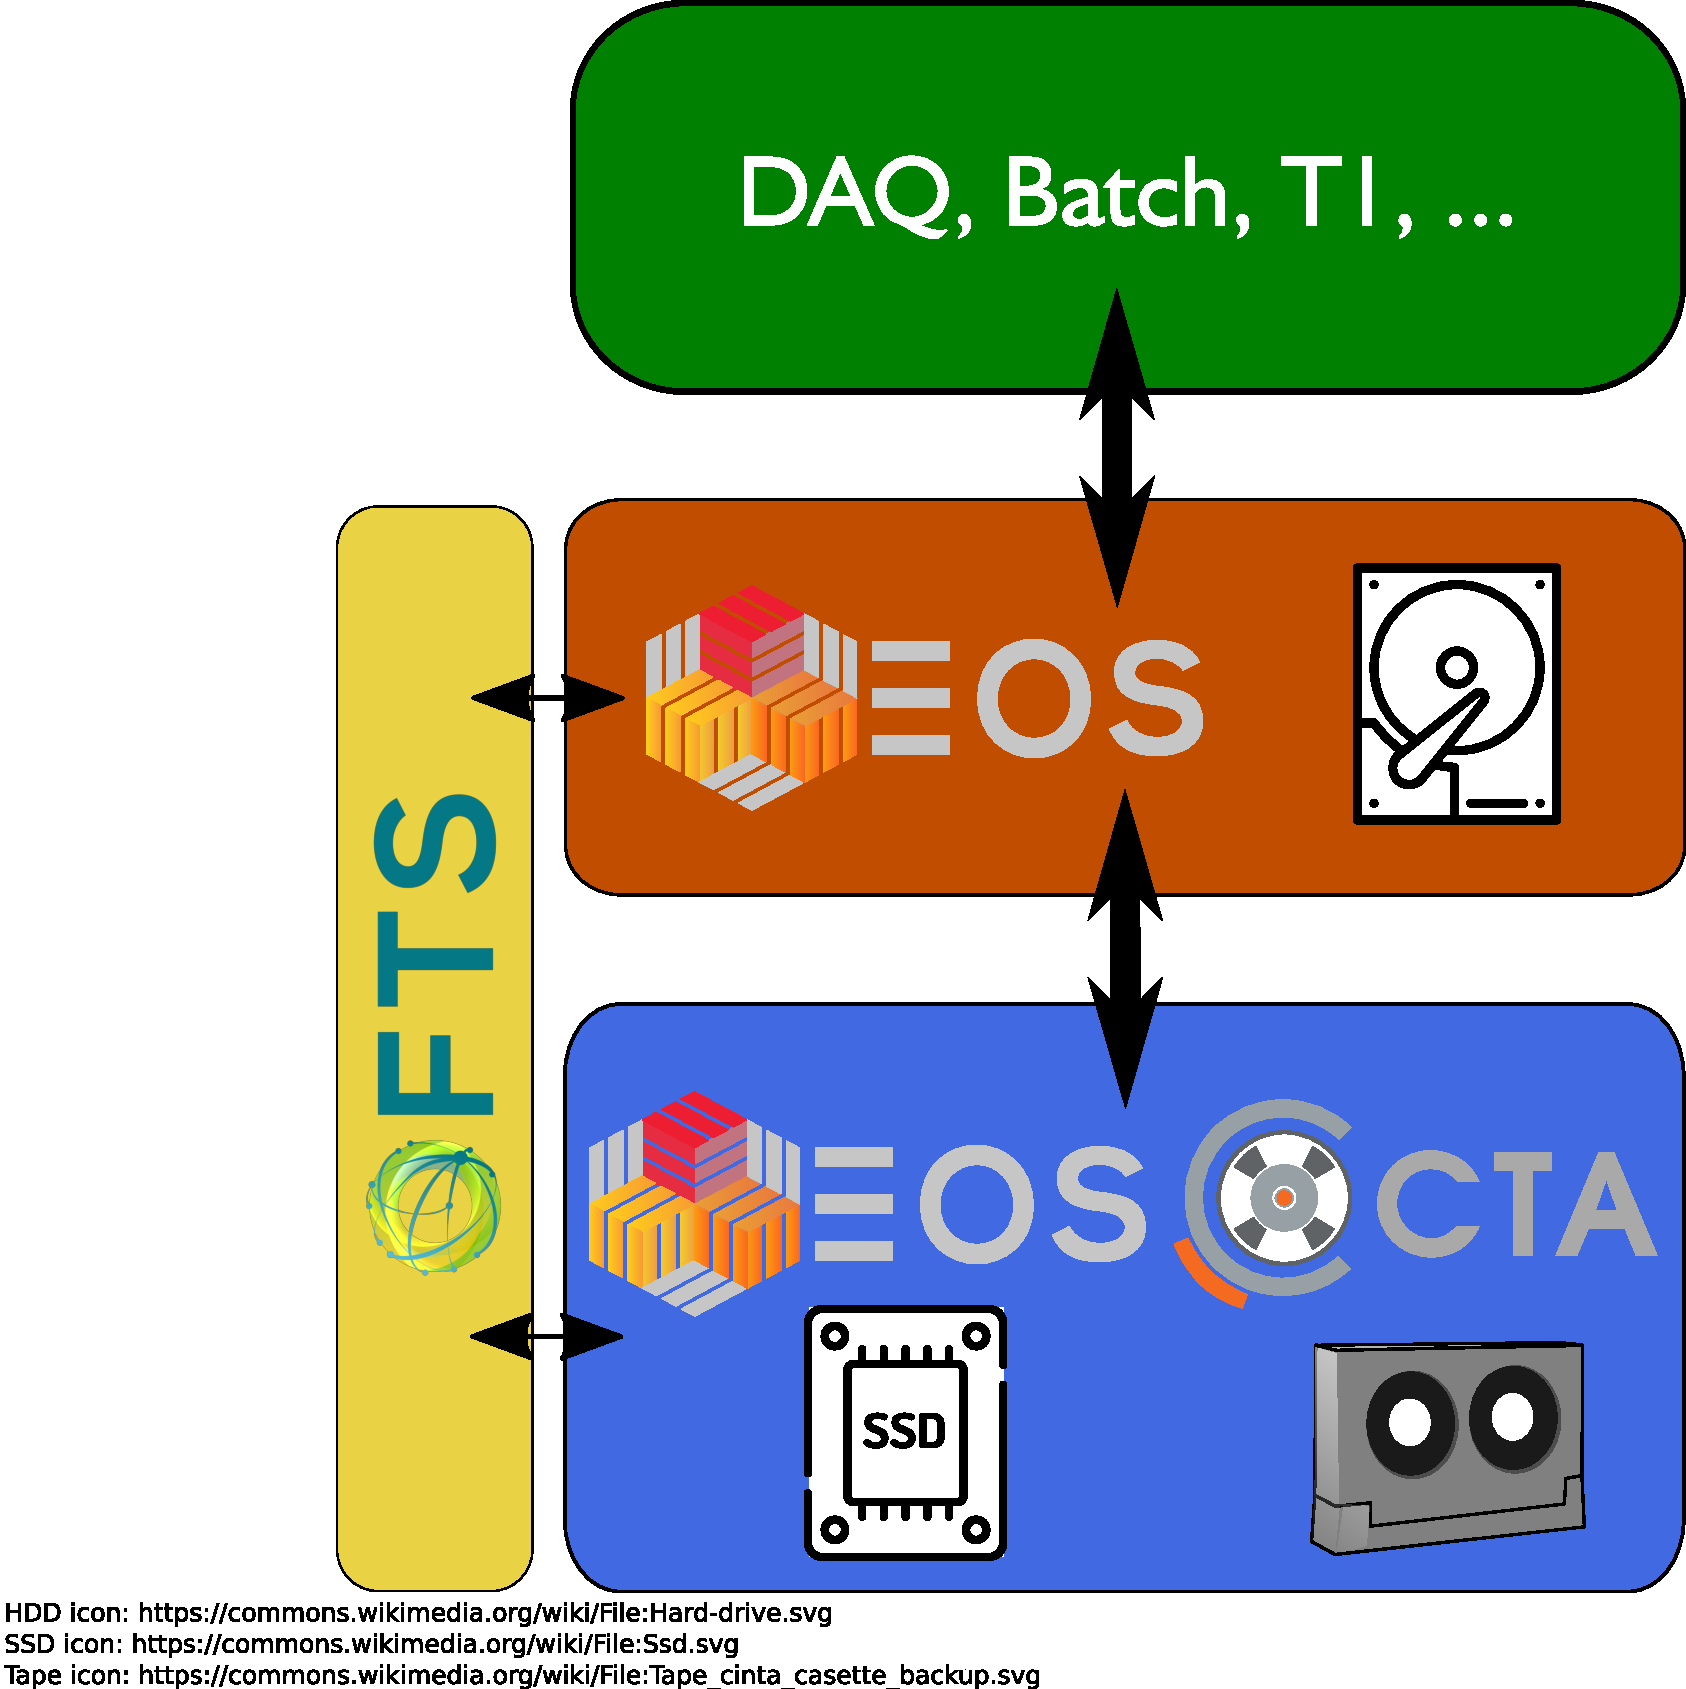
\includegraphics[width=\textwidth]{images/CTA_Deployment_small}
		\end{center}
	\end{column}
	\begin{column}{0.55\textwidth}
		We will contact you in the coming months to :
		\begin{itemize}
		  \item Understand your data management workflows
        \item Discuss the best time to schedule the migration from CASTOR to CTA
		\end{itemize}
	\end{column}
\end{columns}
\end{frame}

\begin{frame}{EOS+CTA Status : Summary}{}
\begin{center}

\includegraphics[width=0.5\textwidth]{../../Logo/Logo_EOS+CTA}
\end{center}

\begin{itemize}
    \item Production hardware is installed; software is deployed
    \item ATLAS acceptance testing in March
    \item End 1Q: ATLAS migration CASTOR $\rightarrow$ EOS+CTA
    \item 2Q: ALICE testing and migration CASTOR $\rightarrow$ EOS+CTA
    \item Other LHC experiments to be migrated before YE 2020
    \item Non-LHC experiments will be contacted in the coming months
\end{itemize}
\end{frame}

\backcover

\end{document}
